\section{Diseño de la arquitectura}

\subsection{Cola de mensajes}
 
El mecanismo de comunicación que se utilizó para el pasaje de información entre
los distintos procesos dentro del trabajo práctico, fue la cola de mensages. La 
principal razón por la cual se optó por este mecanismo se debió a que el sincronismo
entre los mensajes escritos y leídos está a cargo del sistema operativo. En un 
principio se pensó en utilizar memoria compartida, sincronizando el acceso a la misma
con semáforos. Esta solución era un poco limitada, ya que acotaba el tamaño de los
datos compartidos a un máximo pre-establecido. En el caso de la tabla de contactos 
se limitaría la cantidad de usuarios registrados y también cuando dos usuarios estuvieran chateando
no podrían enviarse mensajes más extensos que el tamaño de la memoria compartida. Por
otro lado, se analizó la posibilidad de utilizar tuberías con nombre ya que permitían enviar mensajes
de cualquier longitud. El problema en el uso de fifos estaba relacionado con el sincronismo,
ya que es inaceptable que más de un proceso escriba en forma simultánea en la tubería.
Luego de analizar las diferentes alternativas, se optó por utilizar cola de mensajes
ya que era el mecanismo de conumicación que mejor se adaptaba al problema.

\subsection{Arquitectura}
\subsubsection{Cliente-Cliente}
\begin{center}
\small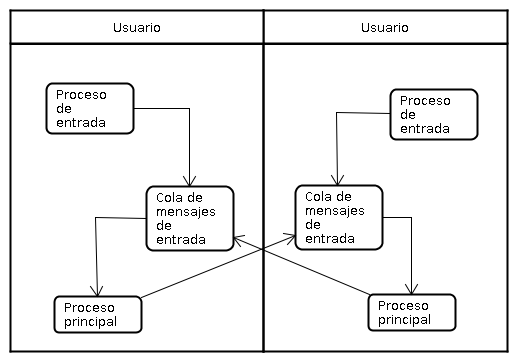
\includegraphics[scale=0.65]{./Images/ArquitecturaClienteConCliente}
\end{center}
\subsubsection{Cliente-Servicio de localización}
\begin{center}
\small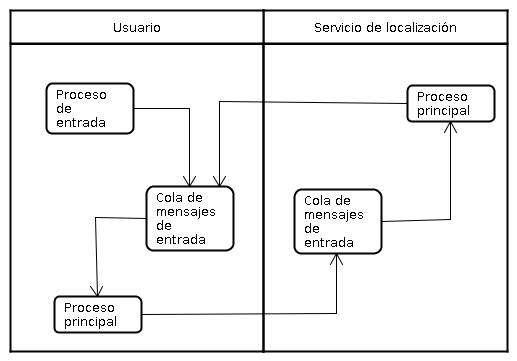
\includegraphics[scale=0.65]{./Images/ArquitecturaClienteConServidor}
\end{center}

\subsection{Diagrama de casos de uso}
\begin{center}
\small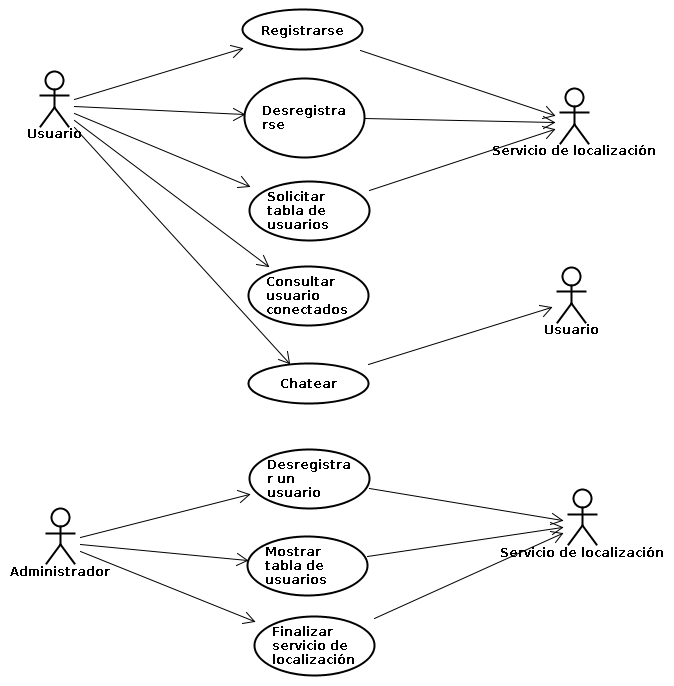
\includegraphics[scale=0.55]{./Images/CasosDeUso}
\end{center}

\subsection{Diagrama de clases}
\begin{center}
\small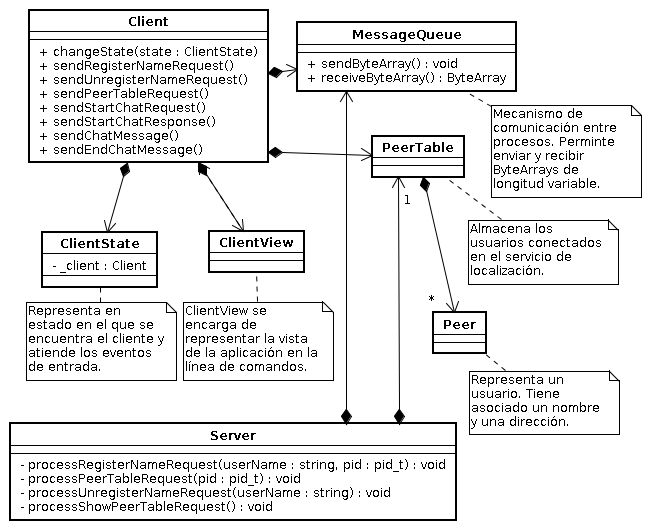
\includegraphics[scale=0.65]{./Images/DiagramaDeClases}
\end{center}

\subsection{Mensajes}

Los procesos se comunican entre sí enviandose mensajes. Se creó una entidad 
llamada ``Message'' la cual encapsula un tipo de mensaje, el id del proceso
creador y los datos asociados el mensaje. Dicho mensaje puede ser serializado
y deserializado para permitir su envio y recepción a través de la cola de mensajes.

\subsubsection{Tipos de mensajes}
\begin{itemize}
  \item {\bf TYPE NONE:} tipo de mensaje inválido.
  \item {\bf TYPE USER INPUT:} enviado desde el proceso que recibe los eventos de teclado \\
hacia el proceso principal cuando el usuario ingresa un comando.
  \item {\bf TYPE USER EXIT:} enviado desde el proceso que recibe los eventos de teclado \\
hacia el proceso principal cuando el usuario ingresa el comando de salida.
  \item {\bf TYPE REGISTER NAME REQUEST:} enviado al servicio de localización para registrar un nuevo usuario.
  \item {\bf TYPE REGISTER NAME RESPONSE:} enviado desde el servicio de localización al usuario para informar \\
si el nombre pudo ser registrado con éxito o no.
  \item {\bf TYPE UNREGISTER NAME REQUEST:} enviado al servicio de localización para desregistrar un usuario.
  \item {\bf TYPE SHOW PEER TABLE REQUEST:} enviado al servicio de localización para hacer que muestre la \\
tabla de contactos.
  \item {\bf TYPE PEER TABLE REQUEST:} enviado al servicio de localización por parte de un usuario para solicitar \\
la tabla de contactos actual.
  \item {\bf TYPE PEER TABLE RESPONSE:} enviado desde el servicio de localización al usuario como respuesta \\
de la solicitud de la tabla de contactos. 
  \item {\bf TYPE START CHAT REQUEST:} enviado entre usuarios para solicitar el comienzo de una seción de chat.
  \item {\bf TYPE START CHAT RESPONSE:} enviado entre usuarios para confirmar o rechazar el inicio de la seción de chat.
  \item {\bf TYPE END CHAT:} enviado entre usuarios para informar el fin de la seción de chat.
  \item {\bf TYPE CHAT MESSAGE:} enviado entre usuarios. Mensaje de chat.
  \item {\bf TYPE SERVER EXIT:} enviado al servicio de localización para cerrarlo remotamente.
\end{itemize}

\subsection{Estados del cliente}

Cada vez que el usuario ingresa un comando, se procesa. El significado de los mensajes o comandos
tipeados por el usuario dependen del estado en el que se encuentre la aplicación al momento de 
enviarlos. Por ejemplo, si dos usuarios se encuentran chateando, y uno usuario ingresa un comando 
``usuarios'' (visualizar la tabla de contactos) se esperaría que el usuario con el que se encuentra
chateando reciba un mensaje en texto plano con el contenido ``usuarios'' y no que visualice la
tabla de contactos en su terminal. Por esta razón, se optó por el uso del patrón de diseño ``State'' 
(o estado) el cual nos permite que cada tipo de estado sea el encargado de procesar los mensajes que llegan 
al proceso principal de cada usuario. 

\subsubsection{Diagrama de estados}
\begin{center}
\small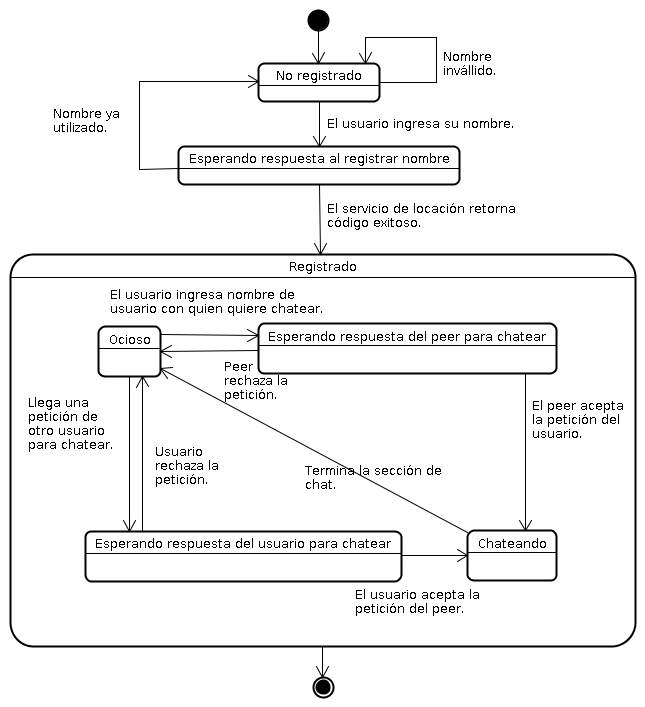
\includegraphics[scale=0.65]{./Images/DiagramaDeEstados}
\end{center}

\subsubsection{Diagrama de clases de los estados}
\begin{center}
\small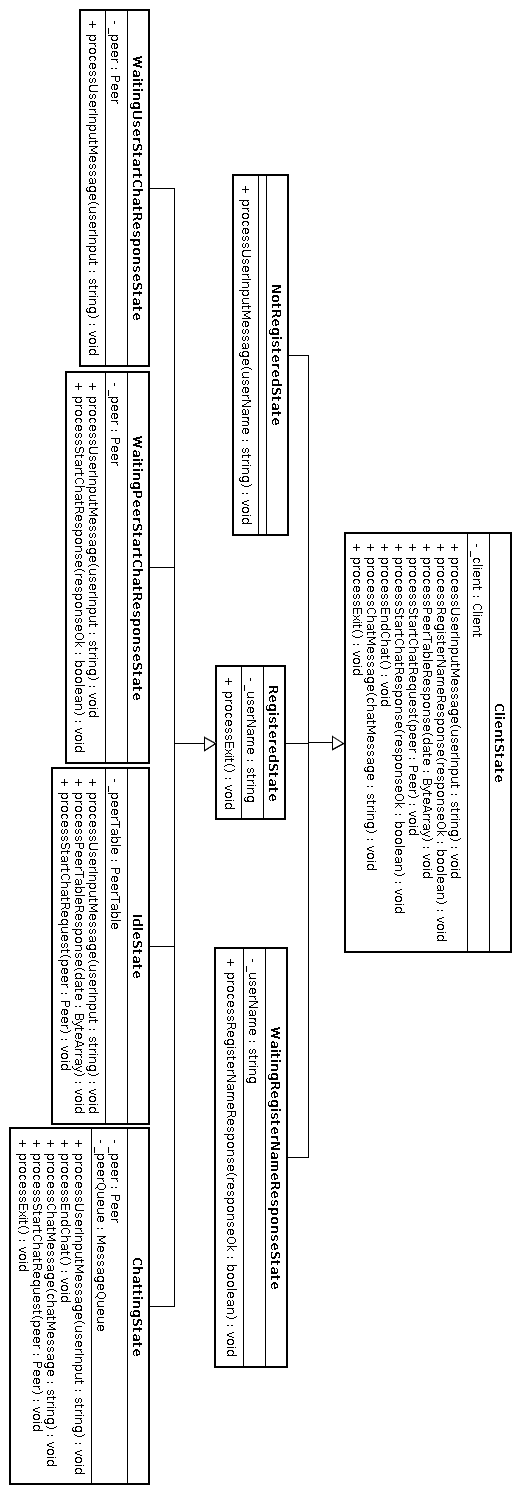
\includegraphics[scale=0.45]{./Images/DiagramaDeClasesDeLosEstados2}
\end{center}

